% \setcounter{section}{0}
\section{Логика и арифметика}

\subsection{Теорема об однозначном представлении булевой функции многочленом Жегалкина}
\textbf{Теорема (Жегалкина):} Каждая булева функция единственным образом представляется в виде полинома Жегалкина.

$\blacktriangle$ Заметим, что различных булевых функций от $n$ переменных $2^{2^n}$ штук. При этом конъюнкций вида $x_{i_1}\ldots x_{i_k}$ существует ровно $2^n$, так как из $n$ возможных сомножителей каждый или входит в конъюнкцию, или нет. В полиноме у каждой такой конъюнкции стоит 0 или 1, то есть существует $2^{2^n}$ различных полиномов Жегалкина от $n$ переменных.

Теперь достаточно лишь доказать, что различные полиномы реализуют различные функции. Предположим противное. Тогда приравняв два различных полинома и перенеся один из них в другую часть равенства, получим полином, тождественно равный нулю и имеющий ненулевые коэффициенты. Тогда рассмотрим слагаемое с единичным коэффициентом наименьшей длины, то есть с наименьшим числом переменных, входящих в него (любой один, если таких несколько). Подставив единицы на места этих переменных и нули на места остальных, получим, что на этом наборе только одно это слагаемое принимает единичное значение, то есть нулевая функция на одном из наборов принимает значение 1. Противоречие. Значит, каждая булева функция реализуется полиномом Жегалкина единственным образом. $\quad \blacksquare$ 

\subsection{Теорема о дедукции для исчисления высказываний}

\textbf{Теорема о дедукции:} Пусть $\Gamma$, $A$ -- это $\Gamma \,\cup\, \{A\}$, тогда верно:
$$\frac{\Gamma\vdash A\to B}{\Gamma,A\vdash B}\;\;\Updownarrow$$

$\blacktriangle$ $(\,\Downarrow)$ Пусть $\Gamma \vdash A\to B$, тогда $\Gamma, A \vdash A,\; A\to B$. К выводу применим MP: $A,\;A\to B \vdash B$. Тогда по транзитивности $\Gamma, A\vdash B$. \newline $(\,\Uparrow)$ Доказывается индукцией по длине вывода $B$ из $\Gamma, A$
\begin{itemize}
    \item[(1)] Если этот вывод -- длины $1$, то $B$ -- аксиома или гипотеза (т.е. формула из $\Gamma$). \newline Если B -- аксиома, то имеем вывод $A \to B$ (из $\O$): \newline 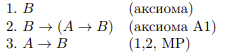
\includegraphics[width=0.35\linewidth]{images/1.1_case1.png}
    \item[(2)] Если $B \in \Gamma$, то имеем такой же вывод $A \to B$ из $\Gamma$: \newline 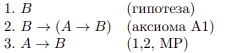
\includegraphics[width=0.35\linewidth]{images/1.1_case2.png}
    \item[(3)] Если $B = A$, то $A \to B = A \to A$. Но $\vdash A \to A$ (пример из определений в пункте 6).
    \item[(4)] Предположим теперь, что $\Gamma, A \vdash B$ и утверждение $(\,\Uparrow)$ верно для всех более коротких выводов, т.е. \newline для всех $C$, если $\Gamma, A \vdash C$ и вывод $C$ из $\Gamma$, $A$ короче, чем вывод $B$, то $\Gamma$ $\vdash A \to C$.
    \newline Докажем, что $\Gamma \vdash A \to B$:
    \newline Рассмотрим вывод из $\Gamma, A$, который заканчивается формулой $B$. При этом $B$ может оказаться аксиомой или гипотезой (тогда все предыдущие формулы для доказательства $B$ не нужны). Но в этом случае  $\Gamma \vdash A \to B$ по (1)–(3).
    \newline Остается случай, когда $B$ получается по MP из формул $C, C \to B$, причем $\Gamma, A \vdash C$ и $\Gamma, A \vdash C \to B$ с более короткими доказательствами. По предположению индукции имеем: \newline
    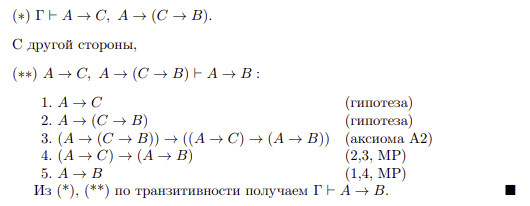
\includegraphics[width=0.9\linewidth]{images/1.1_case3.png}
\end{itemize}

\subsection{Теорема о полноте исчисления высказываний}

Из следующей теоремы нам понадобятся только 4) и 6) правила.
\par

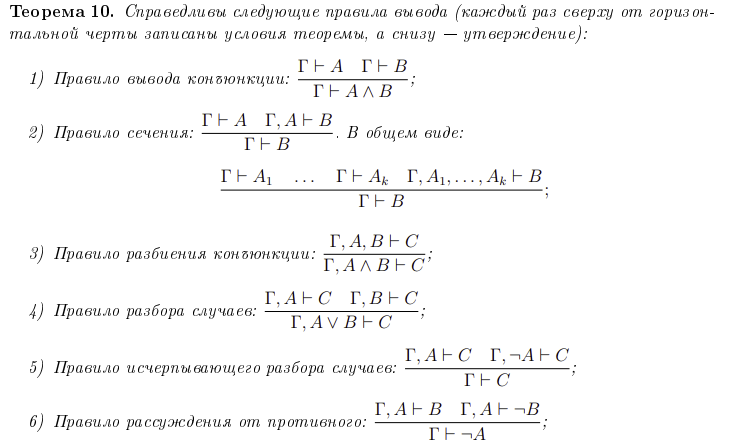
\includegraphics[width=0.97\linewidth]{images/1.2_theorem}

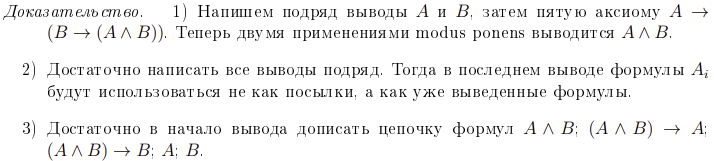
\includegraphics[width=0.95\linewidth]{images/1.1_v1}

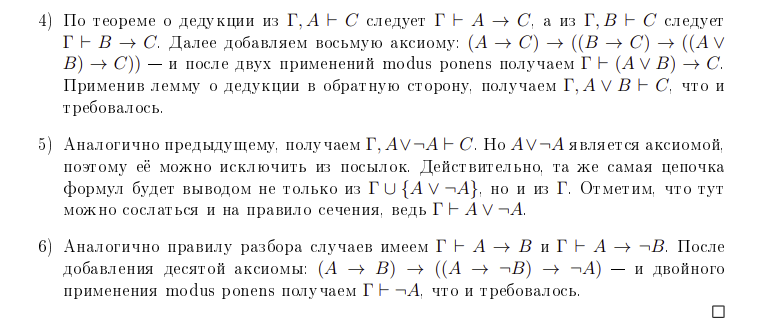
\includegraphics[width=0.95\linewidth]{images/1.1_v3}

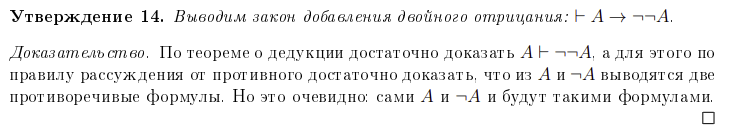
\includegraphics[width=0.95\linewidth]{images/1.1_neg}

\par \noindent Для доказательства теоремы о полноте понадобятся две вспомогательные леммы.

\textbf{Базовая лемма:} Представление таблицы истинности для данных четырех связок.

\begin{tabular}{|p{1.5in}|p{1.5in}|p{1.5in}|p{1.5in}|}
\hline
    Для дизъюнкции: & Для конъюнкции: & Для импликации: & Для отрицания:\\ 
    \hline
    \centering{$A,B \vdash A\lor B$} & \centering{$A,B \vdash A \land B$} & \centering{$A,B \vdash A\to B$} & \centering{$A \vdash \neg (\neg A)$} \tabularnewline
    
    \centering{$\neg A,B \vdash A\lor B$} & \centering{$\neg A,B \vdash \neg (A\land B)$} & \centering{$\neg A,B \vdash A\to B$}& \centering{$\neg A \vdash \neg A$} \tabularnewline
    
    \centering{$A,\neg B \vdash A\lor B$} & \centering{$A, \neg B \vdash \neg (A\land B)$} & \centering{$A,\neg B \vdash \neg (A\to B)$}& \centering{} \tabularnewline
    
    \centering{$\neg A,\neg B \vdash \neg (A\lor B)$} & \centering{$\neg A, \neg B \vdash \neg (A\land B)$} & \centering{$\neg A,\neg B \vdash A\to B$}& \centering{} \tabularnewline
    \hline
\end{tabular}

\begin{enumerate}
    \item Первые три выводимости про дизъюнкцию следуют из $A_6$ и $A_7$ по лемме о дедукции ($D$). Последняя: \newline
    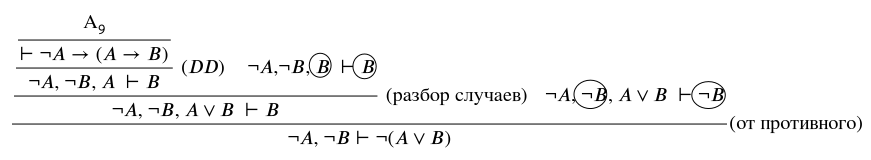
\includegraphics[width=0.99\linewidth]{images/1.1_dedu.png}
    \item Первая выводимость про конъюнкцию следует из $A_5$ по $D$, остальные получаются контрапозицией из $A_3$ и $A_4$: \newline
    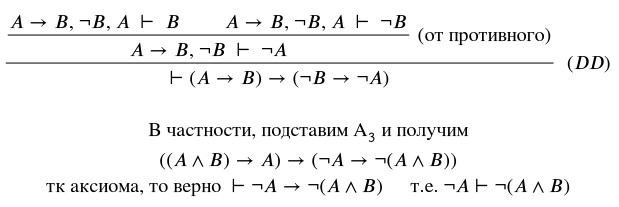
\includegraphics[width=0.8\linewidth]{images/1.1_cntrl.png}
    \item Первая, третья и четвертая выводимость про импликацию следуют из $A_1$ и $A_9$ по $D$. Вторая выводится так: \newline
    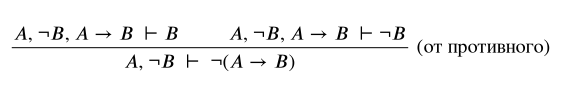
\includegraphics[width=0.7\linewidth]{images/1.1_negg.png}
    \item Первая выводимость про отрицание доказана в утверждении 14, вторая тривиальна.
\end{enumerate}

\par \textbf{Основная лемма:} Пусть $\phi$ - это формула, зависящая от $p_1,\ldots,p_n$. Тогда верно следующее:
$$p_1^{a_1},p_2^{a_2},\ldots,p_n^{a_n} \vdash \phi^{\phi(a_1,\ldots,a_n)} \text{, \qquad где } p^a = \begin{cases}
p, a = 1\\
\neg p, a = 0
\end{cases}$$
Обозначим $a = \phi(a_1,\ldots,a_n)$

$\blacktriangle$ Доказательство будет вестись индукцией по построению формулы с использованием базовой леммы в качестве базы и в переходе.
\newline \textit{База индекции:} $\phi$ содержит  одну связку. Тогда это утверждение сводится к базовой лемме.
\newline \textit{Переход:} пусть $\phi = \psi \land \gamma$. Тогда можно записать: $\phi(a_1,\ldots,a_n) = \psi(a_1,\ldots,a_n) \land \gamma(a_1,\ldots,a_n)$
\newline Пусть $\psi(a_1,\ldots,a_n) = \alpha, \;\; \gamma(a_1,\ldots,a_n) = \beta$
\newline Применим предположение индукции: $p_1^{a_1},\ldots,p_n^{a_n} \vdash \psi^\alpha, \;\;\; p_1^{a_1},\ldots,p_n^{a_n} \vdash \gamma^\beta$
\newline Воспользуемся базовой леммой:
$\psi^\alpha, \; \gamma^\beta \vdash (\psi \land \gamma)^{(\alpha\land\beta)}=\phi^a $
\newline Записав все выводы подряд, получаем: $p_1^{a_1},p_2^{a_2},\ldots,p_n^{a_n} \vdash \phi^{a}$
\newline Аналогичные действия проделаем и для других связок. Имеются база и переход, значит, по индукции докажем лемму для всех формул. $\qquad \blacksquare$

\textit{Пример:} $\phi=\neg p \land (q\lor r); \quad \phi(0,1,0)=1;\quad \phi(1,0,0)=1$

Лемма утверждает следующее: $\quad \neg p, q, \neg r \vdash \phi; \qquad p, \neg q, \neg r \vdash \neg \phi$
\newline \par \textbf{Теорема о полноте ИВ:} Если формула $\phi$ является тавтологией, то тогда $\phi$ -- выводима. 

$\blacktriangle$ Пусть $\phi$ -- тавтология. Тогда $\forall a_1\ldots a_n \;\; \phi(a_1,\ldots,a_n) = 1$. Значит, по основной лемме $ p_1^{a_1},p_2^{a_2},\ldots,p_n^{a_n} \vdash \phi$ при $\forall a_1\ldots a_n$. Далее воспользуемся правилом исчерпывающего разбора случаев, а также закон исключенного третьего: \newline
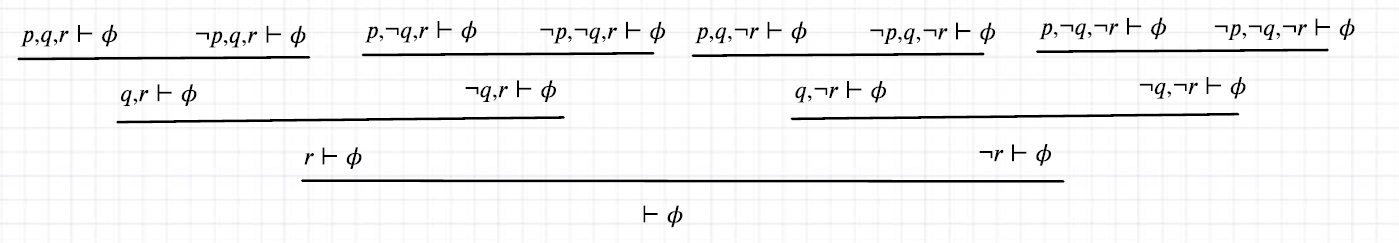
\includegraphics[width=1\linewidth]{images/1.1_cases.png}
Такое рассуждение можно провести не только для трех литералов, но и для любого количества. Значит, теорема о полноте доказана. $\qquad \blacksquare$